\documentclass{article}
\usepackage{fancyhdr}
\usepackage{ctex}
\usepackage{listings}
\usepackage{graphicx}
\usepackage[a4paper, body={18cm,22cm}]{geometry}
\usepackage{amsmath,amssymb,amstext,enumerate,graphicx}
\usepackage{float,abstract,booktabs,indentfirst,amsmath}
\usepackage{array}
\usepackage{booktabs}
\usepackage{multirow}
\usepackage{url}
\usepackage{diagbox}
\renewcommand\arraystretch{1.4}
\usepackage{indentfirst}
\setlength{\parindent}{2em}
\usepackage{enumerate}
\setmonofont{Consolas}
\usepackage{listings}
\usepackage{xcolor}
\usepackage{makecell}
\usepackage{enumitem}
\usepackage{tikz}
\usepackage{wrapfig}
\usepackage{tkz-euclide}
\usepackage{pgfplots}
\usepackage{multicol}
\setfontfamily{\timesfont}{Times New Roman}

\begin{document}

\newcommand{\titem}[1]{
~\\
\begin{itemize}
    \item \heiti \large {#1}
\end{itemize}
}

\newcommand{\bb}[1]{{\heiti {#1}}}

\renewcommand{\d}{\mathrm{d}}

\newcommand{\cf}[1]{$^{#1}\textrm{C}$}

\title{《数学建模及其MATLAB实现》第六次课程作业}
\author{李鹏达}
    

\begin{center}
    \LARGE \textbf{\heiti 《数学建模及其{\timesfont MATLAB}实现》第七次课程作业} \\[0.5em]
    \large 李鹏达 10225101460
\end{center}

~\\

\paragraph{1.}在食饵-捕食者系统中,如果在食饵方程
    \(
    \dot{x}(t) = x \left( r - ay \right) = rx - axy
    \)
    中增加自身阻滞作用的 logistic 项,而方程
    \(
    \dot{y}(t) = y \left( -d + bx \right) = -dy + bxy
    \)
    不变,讨论平衡点及稳定性,解释其意义.\\

\noindent\textbf{{\heiti 解答:}}

    食饵方程中增加自身阻滞作用的 logistic 项,将增长率 $r$ 替换为 $r(x) = r^* \left(1- \frac{x}{N} \right)$,其中 $r^*$ 为最大增长率, $N$ 为环境容纳.则食饵方程变为
    \[
    \dot{x}(t) = x \left[ r^* \left( 1 - \frac{x}{N} \right) - ay \right] = r^* x - \frac{r^*}{N} x^2 - axy
    \]

    微分方程组变为
    \[
    \begin{cases}
        \dot{x}(t) = r^* x - \frac{r^*}{N} x^2 - axy \\
        \dot{y}(t) = -dy + bxy
    \end{cases}
    \]

    令 $\dot{x} = \dot{y} = 0$,解方程组
    \[
    \begin{cases}
        r^* x - \frac{r^*}{N} x^2 - axy = 0 \\
        -dy + bxy = 0
    \end{cases}
    \]

    得平衡点 $P_1(0,0)$, $P_2(N, 0)$, $P_3(\frac{d}{b}, \frac{r^*}{a}(1- \frac{d}{bN}))$.

    方程组的系数矩阵
    \[
    A = \begin{bmatrix}
        r^* - \frac{2r^*}{N} x - ay & -ax \\
        by & bx - d
    \end{bmatrix}
    \]

    (1)对于平衡点 $P_1(0,0)$, 
    \[
    A|_{P_1} = \begin{bmatrix}
        r^* & 0 \\
        0 & -d
    \end{bmatrix}
    \]

    $q=-r^*d < 0$,故平衡点 $P_1$ 是不稳定的.

    (2)对于平衡点 $P_2(N,0)$,
    \[
    A|_{P_2} = \begin{bmatrix}
        -r^* & -aN \\
        0 & bN - d
    \end{bmatrix}
    \]

    $p=r^*-(bN-d)$, $q=-r^*(bN-d)$.
    
    此时,稳定条件为 $bN-d < 0$.这说明了当食饵的种群数量达到环境容纳量时,捕食者的增长率$y (bN-d)$仍小于$0$,食饵的种群数量达到最大值也不能供养捕食者,最终达到一个食饵数量维持在环境容纳量、捕食者灭绝的稳定状态.

    (3)对于平衡点 $P_3(\frac{d}{b}, \frac{r^*}{a}(1- \frac{d}{bN}))$,
    \[
    A|_{P_3} = \begin{bmatrix}
        -\frac{dr^*}{bN} & -\frac{ad}{b} \\
        \frac{r^*}{a}\left(b-\frac{d}{N}\right) & 0
    \end{bmatrix}
    \]

    $p=\frac{dr^*}{bN} > 0$, $q=\frac{dr^*}{b}\left(b-\frac{d}{N}\right)$.

    此时,稳定条件为 $b-\frac{d}{N}>0$,即 $bN-d>0$.这说明了当食饵的种群数量达到环境容纳量时,捕食者的增长率$y (bN-d)$大于$0$,食饵的种群数量达到最大值时可以供养捕食者,最终达到一个食饵数量维持在一个稳定值、捕食者数量维持在一个稳定值的稳定状态.\\

    在这种情况下,由于我们给食饵引入了自身阻滞作用,使得食饵不在无限制地增长,系统最后达到的平衡状态取决于食饵能否供养捕食者.若食饵不能供养捕食者,则最终食饵数量维持在环境容纳量,捕食者灭绝;若食饵能供养捕食者,则最终食饵数量维持在一个稳定值,捕食者数量维持在一个稳定值.\\
~\\

\paragraph{2.}如果在食饵和捕食者方程中都增加 logistic 项,即下列方程,讨论平衡点及稳定性.
    \[
    \begin{cases}
        \dot{x}_1(t) = r_1 x_1 \left( 1 - \frac{x_1}{N_1} - \sigma_1 \frac{x_2}{N_2} \right) \\
        \dot{x}_2(t) = r_2 x_2 \left( -1 + \sigma_2 \frac{x_1}{N_1} - \frac{x_2}{N_2} \right)
    \end{cases}
    \]

\noindent\textbf{{\heiti 解答:}}

    令 $\dot{x}_1 = \dot{x}_2 = 0$,解方程组
    \[
    \begin{cases}
        r_1 x_1 \left( 1 - \frac{x_1}{N_1} - \sigma_1 \frac{x_2}{N_2} \right) = 0 \\
        r_2 x_2 \left( -1 + \sigma_2 \frac{x_1}{N_1} - \frac{x_2}{N_2} \right) = 0
    \end{cases}
    \]

    得平衡点 $P_1(0,0)$, $P_2(N_1, 0)$, $P_3(\frac{N_1(1+\sigma_1)}{1+\sigma_1\sigma_2},\frac{N_2(\sigma_2-1)}{1+\sigma_1\sigma_2})$.

    方程组的系数矩阵
    \[
    A = \begin{bmatrix}
        r_1 \left( 1 - \frac{2x_1}{N_1} - \sigma_1 \frac{x_2}{N_2} \right) & -\sigma_1 \frac{r_1 x_1}{N_2} \\
        \sigma_2 \frac{r_2 x_2}{N_1} & r_2 \left( -1 + \sigma_2 \frac{x_1}{N_1} - \frac{2x_2}{N_2} \right)
    \end{bmatrix}
    \]

    (1) 对于平衡点 $P_1(0,0)$,
    \[
    A|_{P_1} = \begin{bmatrix}
        r_1 & 0 \\
        0 & -r_2
    \end{bmatrix}
    \]

    $q=-r_1r_2 < 0$,故平衡点 $P_1$ 是不稳定的.

    (2) 对于平衡点 $P_2(N_1,0)$,
    \[
    A|_{P_2} = \begin{bmatrix}
        -r_1 & -\sigma_1 \frac{N_1r_1}{N_2} \\
        0 & r_2(\sigma_2-1)
    \end{bmatrix}
    \]

    $p=r_1-r_2(\sigma_2-1)$, $q=-r_1r_2(\sigma_2-1)$.

    此时,稳定条件为 $\sigma_2-1 < 0$,即 $\sigma_2 < 1$.而$\sigma_2$ 反映的使食饵供养捕食者的能力,当 $\sigma_2 < 1$ 时,食饵不能供养捕食者,最终达到一个食饵数量维持在环境容纳量、捕食者灭绝的平衡状态.

    (3) 对于平衡点 $P_3(\frac{N_1(1+\sigma_1)}{1+\sigma_1\sigma_2},\frac{N_2(\sigma_2-1)}{1+\sigma_1\sigma_2})$,
    \[
    A|_{P_3} = \begin{bmatrix}
        -\frac{r_1(\sigma_1 + 1)}{1+\sigma_1\sigma_2} & -\frac{\sigma_1r_1N_1(1+\sigma_1)}{N_2(1+\sigma_1\sigma_2)} \\
        \frac{r_2\sigma_2N_2(\sigma_2-1)}{N_1(1+\sigma_1\sigma_2)} & -\frac{r_2(\sigma_2-1)}{1+\sigma_1\sigma_2}
    \end{bmatrix}
    \]

    $p=\frac{r_1(\sigma_1 + 1)+r_2(\sigma_2-1)}{1+\sigma_1\sigma_2} > 0$, $q=\frac{r_1r_2(\sigma_2-1)(\sigma_1+1)}{(1+\sigma_1\sigma_2)}$.

    此时,稳定条件为 $\sigma_2-1 > 0$,即 $\sigma_2 > 1$.而$\sigma_2$ 反映的使食饵供养捕食者的能力,当 $\sigma_2 > 1$ 时,食饵能供养捕食者,最终达到一个食饵数量维持在一个稳定值、捕食者数量维持在一个稳定值的平衡状态.\\

    在这种情况下,由于我们给食饵和捕食者都引入了自身阻滞作用,使得食饵和捕食者都不在无限制地增长,系统最后达到的平衡状态取决于食饵对捕食者的供养能力 $\sigma_2$.若$\sigma_2 < 1$,食饵不能供养捕食者,则最终食饵数量维持在环境容纳量,捕食者灭绝;若$\sigma_2 > 1$,食饵能供养捕食者,则最终食饵数量维持在一个稳定值,捕食者数量维持在一个稳定值.\\
~\\

\paragraph{3.}在 SIR 模型中设定不同的参数 $\lambda, \mu$ 和初始值 $s(0), i(0)$,编程计算 $s(t)$ 和 $i(t)$ 并作图.需包含 $\sigma s(0) > 1$ 和 $\sigma s(0) < 1$ 的设定,分析这两种情况下患者比例 $i(t)$ 的不同变化.

\begin{enumerate}[label=(\arabic*)]
    \item $\sigma s(0) > 1$
    
    选取的参数为 $\lambda = 0.5, \mu = 0.1, s(0) = 0.8, i(0) = 0.2$.
    
    \begin{figure}[H]
    \centering
    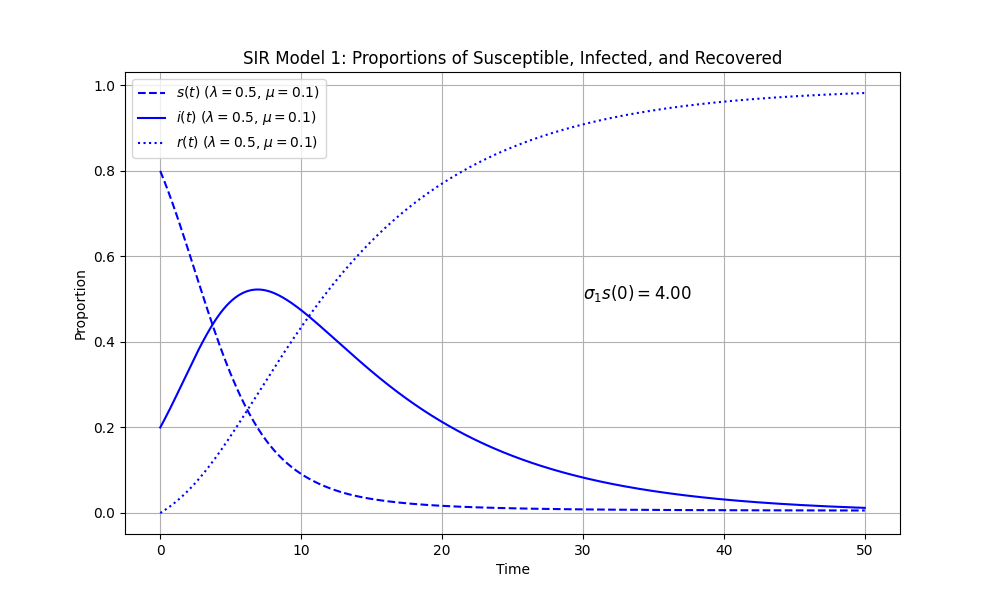
\includegraphics[width=0.7\textwidth]{img/1.png}
    \caption{$\sigma s(0) > 1$}
    \end{figure}

    从图中可以看出,当 $\sigma s(0) > 1$ 时,患者比例 $i(t)$ 随时间的增加先增加后减少,最终趋于0.这是因为当 $\sigma s(0) > 1$ 时,疾病传播速度大于恢复速度,疾病会迅速传播,但随着患者的增多,易感者的数量减少,疾病传播速度减慢,最终感染者数量减少到0.

    \item $\sigma s(0) < 1$
    
    选取的参数为 $\lambda = 0.05, \mu = 0.1, s(0) = 0.8, i(0) = 0.2$.

    \begin{figure}[H]
    \centering
    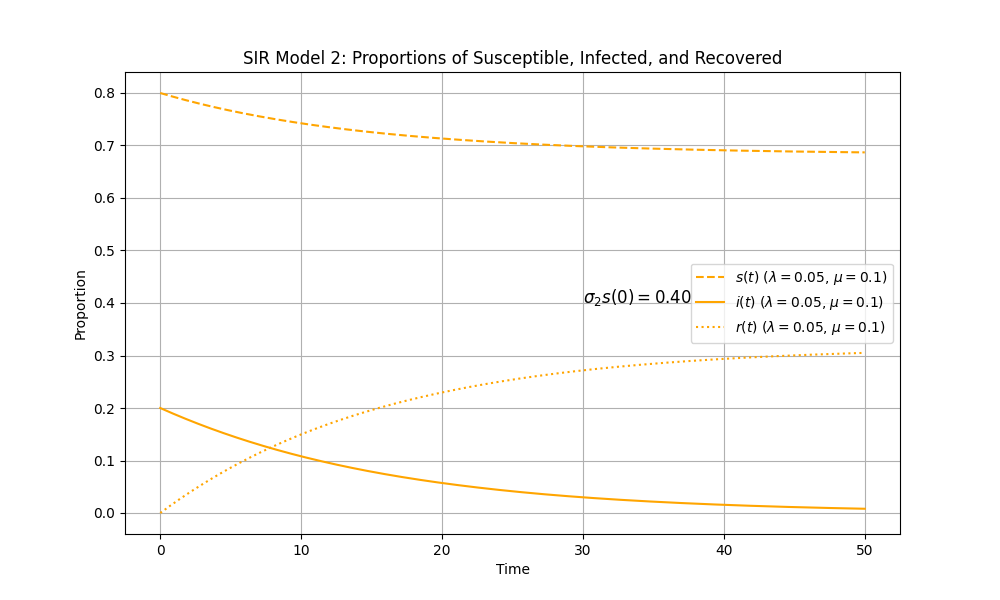
\includegraphics[width=0.7\textwidth]{img/2.png}
    \caption{$\sigma s(0) < 1$}
    \end{figure}

    从图中可以看出,当 $\sigma s(0) < 1$ 时,患者比例 $i(t)$ 随时间的增加先增加后减少,最终趋于0.这是因为当 $\sigma s(0) < 1$ 时,疾病传播速度小于恢复速度,疾病传播缓慢,疾病无法蔓延,患者比例逐渐减少,最终感染者数量减少到0.

\end{enumerate}

\end{document}